\begin{pastexam}[label={px:gk3-100-ds-02}]{高考三級資訊處理 100 年 第二題}
（申論；10 分）

輸入運算式（expression）為 \texttt{-A-(B+C)*D\textasciicircum E}，請畫出其對應之運算樹（expression tree）。
（10 分）
\end{pastexam}

\begin{pastsoln}
答案：根是減號，左子樹是 $-A$（單元負號），右子樹是 $(B+C)*(D\,\hat{}\,E)$，樹畫在下面。

\textbf{先加括號。} 開頭的「\texttt{-}」前面沒有運算元，是\textbf{單元負號}（unary minus），只作用在
$A$ 上。 優先順序由高到低是：單元負號、\texttt{\textasciicircum}（次方）、\texttt{*}、二元的
\texttt{-}。 所以
\[
\texttt{-A-(B+C)*D\textasciicircum E} \;=\; \bigl(-A\bigr) - \Bigl( (B + C) * \bigl(D\,\hat{}\,E\bigr) \Bigr).
\]
最後才做的運算是中間那個二元減號，它就是根；左運算元 $-A$、右運算元 $(B+C)*(D\,\hat{}\,E)$ 再各自
照同樣的方法拆（資結書第~7.7~節）。

\textbf{運算樹。} 運算子是內部節點，運算元是葉子。 單元負號只有一個運算元，所以節點只有一個子節點；
這裡把 $A$ 放在右邊，中序走訪時才會先印「$-$」再印「$A$」，和原式一致。
\begin{center}
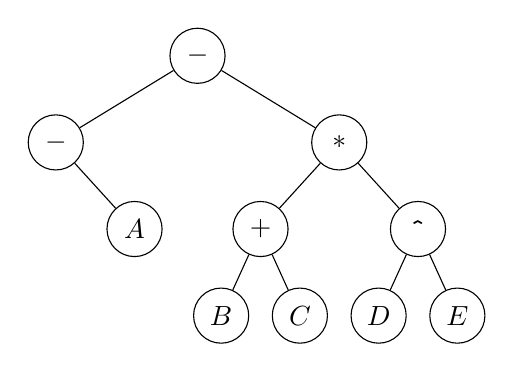
\begin{tikzpicture}[every node/.style={circle,draw,minimum size=7mm,inner sep=0pt},
  level distance=11mm, level 1/.style={sibling distance=36mm}, level 2/.style={sibling distance=20mm},
  level 3/.style={sibling distance=10mm}]
\node {$-$}
  child {node {$-$}
    child[missing]
    child {node {$A$}}}
  child {node {$*$}
    child {node {$+$} child {node {$B$}} child {node {$C$}}}
    child {node {\texttt{\textasciicircum}} child {node {$D$}} child {node {$E$}}}};
\end{tikzpicture}
\end{center}
左邊那個「$-$」是單元負號，右邊樹根的「$-$」是二元減號。 這棵樹的前序是
$-\ (-)\ A\ *\ +\ B\ C\ \hat{}\ D\ E$，後序是 $A\ (-)\ B\ C\ +\ D\ E\ \hat{}\ *\ -$（括號標的是單元負號）；
中序加上括號就回到原式。
\end{pastsoln}
